%\newpage
\subsection{Tecnologie e scelte relative al progetto}
	L'obiettivo di questo paragrafo è descrivere in maniera specifica come \progetto\ andrà a interfacciarsi con le tecnologie.\\
	Per ciascuna di queste è previsto un \gloss{microservizio}, il quale avrà come scopo quello di fare da tramite tra lo strumento che genera il messaggio e quello che lo riceve.\\
	Questo pattern si chiama \gloss{Publisher / Subscriber} e utilizza uno strumento intermedio detto Broker per lo smistamento dei messaggi e la gestione dei flussi.

	\begin{figure}[H]
		\centering
		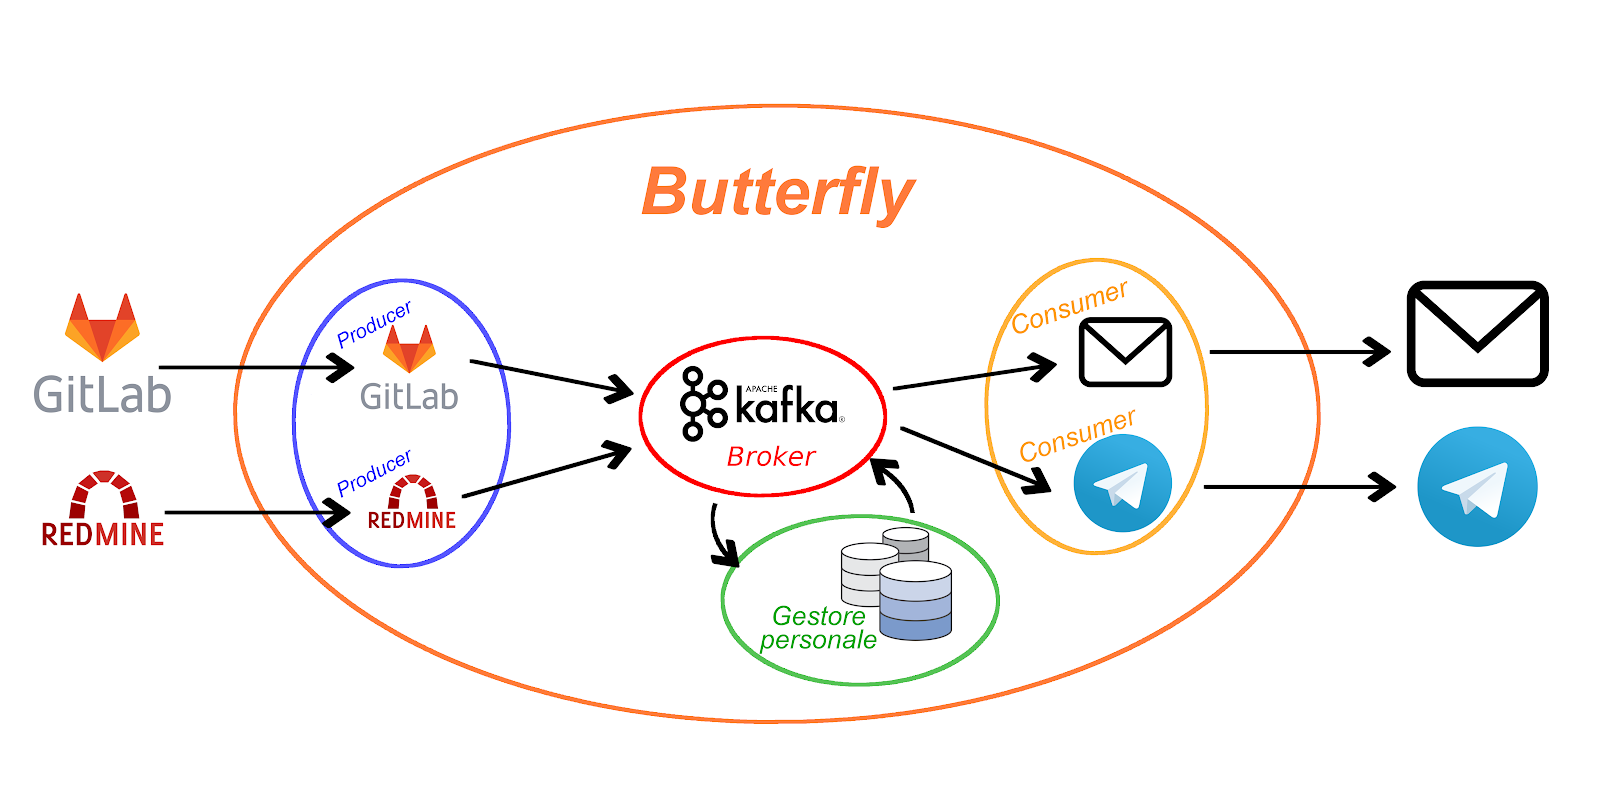
\includegraphics[width=\textwidth]{img/butterfly.png}\\
		\caption{Visione generale del sistema \progetto}
		\label{fig:butterfly}
	\end{figure}
	L'immagine precedente rappresenta una suddivisione del sistema in quattro sezioni principali:
	\begin{itemize}
		\item \progetto\ (arancione)
		\item Producer (azzurro)
		\item Broker (rosso)
		\item Consumer (verde)
	\end{itemize}
	Questa scomposizione ci ha permesso di analizzare più approfonditamente i vari sottosistemi del prodotto in rapporto alle tecnologie esterne a Butterfly (GitLab, Redmine, Telegram ed e-mail), ai microservizi interni come i Producer / Consumer associati e il Broker.
	
	\subsubsection{Producer}\label{TecnologieProducer}
	
		Per ciascuno degli strumenti che invia messaggi verso il sistema è necessario creare una componente applicativa di tipo Producer che li riceva e li elabori inoltrandoli successivamente verso il Broker.
		Le tecnologie dalle quali vengono ricevuti i messaggi sono elencate di seguito in ordine di priorità in base a quanto richiesto dal \gloss{committente}.
		\begin{enumerate}
			\item Redmine
			\item GitLab
			\item SonarQube
		\end{enumerate}
		Abbiamo scelto di sviluppare i Producer per le prime due applicazioni in base alle priorità suggerite da \II\ nel capitolato, lasciando l'applicativo relativo a SonarQube come opzionale.
		Ciascun messaggio ricevuto da queste tecnologie verrà analizzato dal Producer associato in modo da inserirli nel Topic appropriato.\\
		In particolare, le modifiche relative alla \gloss{repository} (GitLab) o al progetto (Redmine) prese in considerazione sono:
		\begin{itemize}
			\item Commit (solo GitLab)
			\item Apertura \gloss{issue} 
			\item Chiusura issue (solo GitLab)
		\end{itemize}
		Le segnalazioni sono generate in base alle \gloss{keyword} contenute nei messaggi di commit e nelle etichette assegnate alle issue.
		Da quest'ultime verrà creato il Topic corrispondente in caso non sia già esistente.
		
		\paragraph{Redmine}
		Ciascuna istanza di Redmine permette l'utilizzo di webhook\footnote{Riferirsi alla voce ``Webhook di Redmine'' alla sezione \S\ref{sec:RiferimentiInformativi}} che inviano segnalazioni al Producer alla modifica del progetto.
		Queste vengono ricevute dal server tramite un microservizio che resta in ascolto, aggiornando in base a quello che riceve i dati presenti sul gestore personale e inoltrando le notifiche ai Consumer interessati.
		
		\paragraph{GitLab}
		Ciascuna istanza di GitLab, online o in un server locale interno dell'azienda, mette a disposizione la configurazione di webhook\footnote{Riferirsi alla voce ``Webhook di GitLab'' alla sezione \S\ref{sec:RiferimentiInformativi}} che, alla modifica della repository, manda un messaggio con le informazioni dei cambiamenti, inseriti nella repository, a un microservizio capace di aggiornare i dati presenti nel gestore personale e, come per Redmine, inoltrare le notifiche ai Consumer interessati.
		
%		\subsubsection{SonarQube}
%		Come GitLab, anche SonarQube prevede l'utilizzo di Webhooks\footnote{\url{https://docs.sonarqube.org/latest/project-administration/Webhooks/}} che dopo ciascuna build comunica il risultato e le informazioni relative ad essa ad un microservizio capace di aggiornare i dati presenti nel gestore personale e, anche in questo caso, inoltrare le notifiche ai customer interessati.
		
	\subsubsection{Broker}\label{TecnologieBroker}
	
		Il ruolo del Broker è quello di smistare i messaggi in base ai Topic con cui questi sono contrassegnati verso i vari microservizi con cui l'utente ha deciso che gli venga inoltrata la notifica.
		L'azienda ci consiglia di utilizzare come Broker per i messaggi \gloss{Apache Kafka}.
	
		\paragraph{Apache Kafka}
		Apache Kafka è un software \gloss{open source} che permette la lettura e la scrittura di messaggi su differenti canali di comunicazioni per i dati.
		Questi messaggi arrivano dai Producer che ricevono le notifiche di applicazioni di terze parti mandandole verso il Broker. Questo le elabora analizzandone il contenuto e contrassegnandole con Topic che verranno utilizzati per l'inoltro ai Consumer e successivamente agli utenti finali, i quali possono abbonarsi a più Topic.
	
	\subsubsection{Consumer}\label{TecnologieConsumer}
		Come per gli strumenti precedentemente elencati, anche per quelli su cui il messaggio andrà ad essere inoltrato, è necessaria la creazione di un microservizio in grado di fare da tramite tra Broker e \gloss{client} dello strumento di messaggistica scelto dall'utente.
		Le tecnologie verso le quali vengono inoltrati i messaggi rielaborati dal sistema sono elencate di seguito in ordine di priorità in base a quanto richiesto dal committente.
		\begin{enumerate}
			\item Telegram
			\item E-mail
			\item Slack
		\end{enumerate}
		Allo stesso modo dei Producer, abbiamo scelto di sviluppare i Consumer per le prime due applicazioni in base alle priorità suggeriteci da \II\ nel capitolato, lasciando l'applicativo relativo a Slack come opzionale.
		Le tecnologie alle quali vengono inoltrati i messaggi sono elencate di seguito in ordine di priorità in base a quanto richiesto dal committente.
			
		\paragraph{Telegram}
		Telegram permette l'interazione in maniera automatica con gli utenti tramite \gloss{bot}\footnote{Riferirsi alla voce ``Bot di Telegram'' alla sezione \S\ref{sec:RiferimentiInformativi}} che possono essere configurati per mandare messaggi ricevuti da strumenti di terze parti, in questo caso \progetto.
		Il Consumer interroga il Broker per acquisire i messaggi da inoltrare e li trasmette effettivamente al bot di Telegram.
		
		\paragraph{E-mail}
		Per inoltrare le e-mail agli utenti finali è necessario che sviluppiamo un Consumer associato che sfrutta un server di posta in modo tale da poter ricevere i messaggi dal Broker e poi mandarli all'indirizzo specificato.
		%https://realpython.com/python-send-email/
		
%		\subsubsection{Slack}
%		È possibile utilizzare le API di Slack per poter mandare push notifications ai canali o alle persone interessate specificando il nome del canale (o lo username della persona), testo del messaggio, e lo username che verrà mostrato per il mittente.
%		%https://www.confluent.io/blog/real-time-syslog-processing-with-apache-kafka-and-ksql-part-2-event-driven-alerting-with-slack/
	
	\subsubsection{Gestore personale}\label{TecnologieGestorePersonale}
	Il gestore personale è quel \gloss{componente} che permette agli utenti di impostare le proprie preferenze per l'applicativo di ricezione dei messaggi ed i Topic a cui si iscrive, interfacciandosi dunque con l'intero sistema \progetto.
	Lo abbiamo previsto come un'applicazione web installata in un server interno all'azienda.
	Questo è accessibile dai dipendenti interessati, i quali potranno quindi modificare, con la possibilità di aggiungere e rimuovere, determinate impostazioni riguardanti le proprie preferenze.
	\newpage
	Quest'ultime sono:
	\begin{itemize}
		\item Scelta dell'applicativo sul quale ricevere le notifiche (Telegram / e-mail)
		\item Iscrizione (o disiscrizione) a determinati Topic
		\item Selezione dei giorni di calendario in cui l'utente segnala la sua assenza
	\end{itemize}
	Nel caso arrivasse una notifica da inoltrare a un utente indisponibile, questa verrà inoltrata alla persona più adatta e disponibile al momento.
	
	\subsubsection{Container software}\label{TecnologieContainer}
	
	Un container software simula un ambiente virtuale dove è possibile testare e mantenere le proprie applicazioni, permettendo di aumentare l'efficienza riducendone i costi e simulando l'esecuzione di sistema operativo su una macchina con \gloss{risorse} condivise.
		
		\paragraph{Differenza tra container e macchina virtuale}
		A differenza delle \gloss{macchine virtuali}, dove lo stato dell'ambiente viene salvato su disco occupando memoria, i container si adattano in maniera più performante all'applicativo richiesto, in quanto il loro scopo è quello di massimizzare la quantità delle applicazioni in esecuzione riducendo al minimo il numero delle macchine per eseguirla.
		Sono quindi più leggeri, occupando meno memoria su disco e impiegando meno risorse.
		%Sebbene.. Purtroppo al termine della loro esecuzione non viene salvato lo stato, a meno che non sia esplicitamente richiesto.
		
		\paragraph{Docker}
		L'azienda ci consiglia di utilizzare \gloss{Docker} per la semplicità di utilizzo e per l'adattamento all'architettura a microservizi.
		La configurazione avverrà tramite un \gloss{Dockerfile} in cui verranno specificate informazioni come sistema operativo, script di avvio, numero di istanze ed altri parametri specifici.

	\subsubsection{Informazioni preconfigurate}
	I dati relativi ai profili esistenti degli utenti presenti nel sistema (ovvero lo username) e le keyword da riconoscere all'interno dei messaggi che vengono ricevuti da GitLab / Redmine, sono considerati già esistenti e presenti nel database del Gestore Personale.
	Questo in quanto non è richiesto da \II\ un sistema di autenticazione, poiché si considera che l'applicativo sia utilizzato internamente all'azienda.
	Non è nemmeno richiesta una configurazione iniziale delle keyword.
	Il progetto quindi non si occupa della gestione dei profili utente in maniera completa e nemmeno di fornire le keyword da riconoscere.
	Per questo motivo non abbiamo pensato a un procedimento di autenticazione tramite la coppia username e password, ma solamente a un username al fine di poter differenziare i diversi utenti.